\chapter{Depth Testing}

Suppose we are drawing more than one object.
To correctly draw them on the screen we have to worry about
the order in which we execute our draw operations.
In particular, to get a realistic image, we must draw
them in descending order based on their distance from the camera.
Although this solution works, it would require us to sort
every object that is going to be rendered by depth.
If there are moving objects, we may have to sort them every frame.
If there are a lot of them, the sorting may require a considerable
amount of time, decreasing the application's framerate.
This solution also causes problems when two objects overlap.
In this case, it's not possible to determine which one
to render first without having graphical artifacts.

An alternative solution that doesn't suffer from the drawbacks
illustrated earlier, is using a depth buffer.
A depth buffer is an image that stores depth data for every pixel.
Every time the rasterizer produces a fragment, the depth test will
check if the new fragment is closer than the previous one.
If it isn't, then the new fragment is discarded.
A fragment that passes the depth test writes its own depth to the
depth buffer.

\begin{figure}[ht]
    \centering
    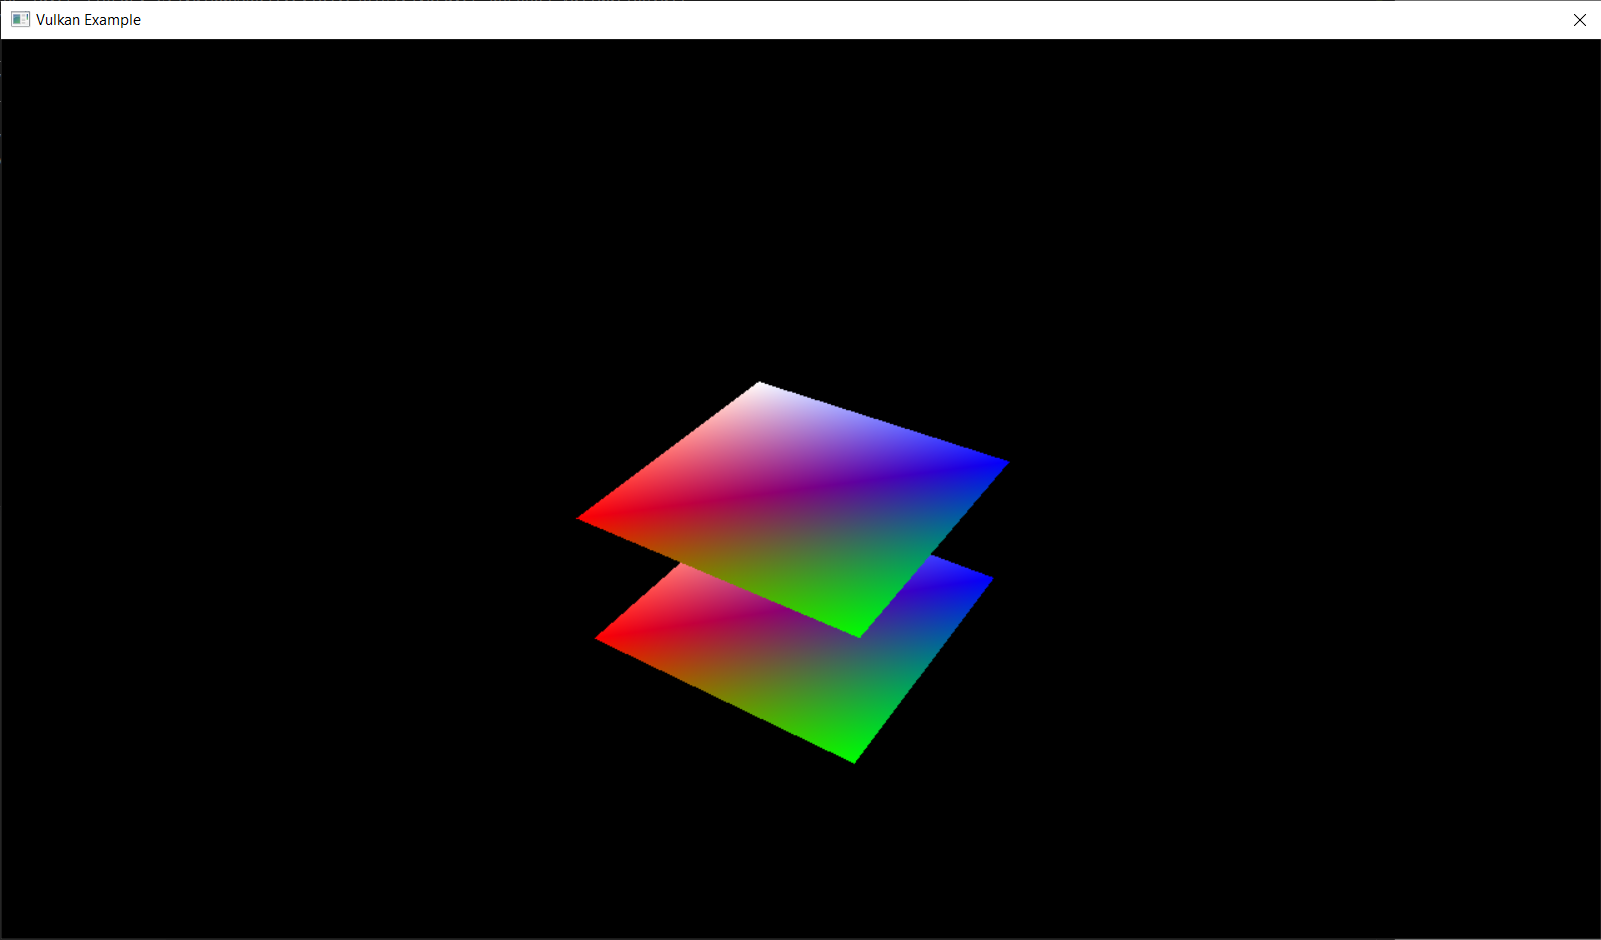
\includegraphics[scale=0.20]{images/ChDepthTesting/DepthTesting.png}
    \caption{Rendering two quads using a depth buffer}
    \label{fig::DepthTesting}
\end{figure}

\section{Creating A Depth Buffer}

Creating a depth buffer means creating an image and using
it as a depth buffer during our rendering operation.
First we must know how to create an image using Vulkan.

\subsection{Creating An Image}

Crating an image in Vulkan consists of four steps.
We first create a \texttt{VkImage} object.
Then, we allocate some memory for our \texttt{VkImage}.
We do this creating a \texttt{VkDeviceMemory} object.
Once we have both the image object and memory, we bind
them together using \texttt{vkBindImageMemory}.
Finally, in order to use the image we have created, we
create a \texttt{VkImageView} on it.

\subsubsection{VkImage}

To create a \texttt{VkImage} we use \texttt{vkCreateImage}.
Here we are creating a 2D image of a given \texttt{width}
and \texttt{height}.
We also specify the image \texttt{format} and \texttt{tiling}.
These two values define the data that the image stores per pixel
and how it's layed out in memory.
Finally, we also specify the image's \texttt{usage}.
The images that we create manually will always be used only
by our graphics queue.
Thus, we use the more performant exclusive sharing mode.

\begin{minipage}{\linewidth}{\noindent}
    \lstinputlisting[
        language=C++,
        caption={Create image object},
        label={lst::CreateImage}
        ]{src/ChDepthTesting/CreateImage.cpp}
\end{minipage}

\texttt{imageType} tells Vulkan with what kind of coordinate
system the pixels in the image are going to be addressed.
\texttt{tiling} can have one of two values: linear or optimal.
With linear tiling, pixels are laid out in row-major order.
With optimal tiling, pixels are laid out in an implementation
defined order for optimal access.
\texttt{usage} has the same semantics as the one during buffer creation.

\subsubsection{VkDeviceMemory}

We allocate some memory for a image object using \texttt{vkAllocateMemory}.
Allocating image memory is the same as allocating buffer memory.

\begin{minipage}{\linewidth}{\noindent}
    \lstinputlisting[
        language=C++,
        caption={Allocate image memory},
        label={lst::AllocateImageMemory}
        ]{src/ChDepthTesting/AllocateImageMemory.cpp}
\end{minipage}

\subsubsection{VkImageView}

We create an image view using \texttt{vkCreateImageView}.
Here, we create a 2D view on an image object, specifying
how to interpret its pixel data and which image aspects
are included in the view.

\begin{minipage}{\linewidth}{\noindent}
    \lstinputlisting[
        language=C++,
        caption={Create image View},
        label={lst::CreateImageView}
        ]{src/ChDepthTesting/CreateImageView.cpp}
\end{minipage}

\texttt{format} is the format and type used to interpret pixels in the image.
\texttt{aspectMask} is a bitmask of \texttt{VkImageAspectFlagBits}
specifying which aspect(s) of the image are included in the view.

\subsection{Cleanup}

We destroy a image view with \texttt{vkDestroyImageView}.
Then we call \texttt{vkDestroyImage} and \texttt{vkFreeMemory}
to clean up the resources we acquired to create an image.

\subsection{Depth Image Creation}

Now that we know how to create an image, we can  create our depth image.
A depth image should have the same resolution as our swapchain images.
It must have an appropriate image usage to be used as a depth buffer.
It should use optimal tiling and have device local memory, supporting fast
read and write operations.
The image should have one of the following formats:
\begin{itemize}
\item \texttt{VK\_FORMAT\_D32\_SFLOAT} using $32$ bits for depth data
\item \texttt{VK\_FORMAT\_D32\_SFLOAT\_S8\_UINT} using $32$ bits for
depth data and $8$ for stencil data
\item \texttt{VK\_FORMAT\_D24\_UNORM\_S8\_UINT} using $24$ bits for
depth data and $8$ for stencil data
\end{itemize}
The most commonly used depth format is \texttt{VK\_FORMAT\_D32\_SFLOAT}.

\begin{minipage}{\linewidth}{\noindent}
    \lstinputlisting[
        language=C++,
        caption={Create Depth Image},
        label={lst::CreateDepthImage}
        ]{src/ChDepthTesting/CreateDepthImage.cpp}
\end{minipage}

\section{Depth Image Render Pass Attachment}

To use our depth buffer we must add it to our render pass as an attachment.

\subsection{VkAttachmentDescription}

Here we describe our depth buffer attachment.
The format should be the same as the depth image itself.
We want to clear it before using it for the first time.
We don't care about storing the depth data, because it will not be
used after drawing has finished.
This may allow the driver to perform additional optimizations.
When our render pass instance begins, we don't care about its previous contents.
Right before finishing our render pass instance, we want its layout to be
optimal for depth stencil operations.

\begin{minipage}{\linewidth}{\noindent}
    \lstinputlisting[
        language=C++,
        caption={Depth buffer render pass attachment description},
        label={lst::DepthBufferRenderPassAttachmentDescription}
        ]{src/ChDepthTesting/DepthBufferRenderPassAttachmentDescription.cpp}
\end{minipage}

\subsection{Attachment descriptions}

Now that we have a new attachment description, we must remember to add it to
oru attachments array.

\begin{minipage}{\linewidth}{\noindent}
    \lstinputlisting[
        language=C++,
        caption={New render pass attachments array},
        label={lst::DepthTestRenderPassAttachments}
        ]{src/ChDepthTesting/DepthTestRenderPassAttachments.cpp}
\end{minipage}

\subsection{Render Pass Subpasses}

Inside our render pass we still have a single subpass.
But, unlike before, not only we have a color attachment, but
we also have a depth stencil attachment.

Here we are saing that our depth image will be used as the subpass depth
stencil attachment.
We are also telling Vulkan to transition our depth buffer image layout to
\texttt{VK\_IMAGE\_LAYOUT\_DEPTH\_STENCIL\_ATTACHMENT\_OPTIMAL} during
this subpass.
We do this because we execute depth operations on our depth image.

\begin{minipage}{\linewidth}{\noindent}
    \lstinputlisting[
        language=C++,
        caption={New render pass subpass},
        label={lst::DepthTestRenderPassSubpass}
        ]{src/ChDepthTesting/DepthTestRenderPassSubpass.cpp}
\end{minipage}

\section{Pipeline Depth Stencil State}

We need to enable depth testing in our pipeline state object.
This is configured through a \texttt{VkPipelineDepthStencilStateCreateInfo}
struct.

Here, we are enabling depth testing.
We are also telling Vulkan to write into the depth buffer the values that
pass the depth test.
We also specify the comparison operation that decides which fragments to
keep and which to discard.
We are sticking to the convention of lower depth means closer to the camera,
so the depth of new fragments should be less.

\begin{minipage}{\linewidth}{\noindent}
    \lstinputlisting[
        language=C++,
        caption={Configure pipeline state depth testing},
        label={lst::EnableVkPipelineDepthStencilStateCreateInfo}
        ]{src/ChDepthTesting/VkPipelineDepthStencilStateCreateInfo.cpp}
\end{minipage}

\section{Depth Image Framebuffer Attachment}

We must remember to add our depth image to the framebuffer we use during
rendering.

\begin{minipage}{\linewidth}{\noindent}
    \lstinputlisting[
        language=C++,
        caption={Modify framebuffer creation},
        label={lst::DepthBufferCreateFramebuffer}
        ]{src/ChDepthTesting/DepthBufferCreateFramebuffer.cpp}
\end{minipage}

\section{Render Pass Clear Values}

Because we now have multiple attachments with
\texttt{VK\_ATTACHMENT\_LOAD\_OP\_CLEAR}, we also need to specify multiple
clear values when we begin our render pass instance.
We clear our color attachment with an opaque black color.
We clear our depth attachment with a depth value of $1.0$.

Depth values range between $0.0$ and $1.0$.
A depth value of $1.0$ means that the fragment is the furthest away from
the camera.
A depth value of $0.0$ means that the fragment is the nearest to
the camera.

\begin{minipage}{\linewidth}{\noindent}
    \lstinputlisting[
        language=C++,
        caption={Render pass clear values},
        label={lst::AttachmentsClearValues}
        ]{src/ChDepthTesting/AttachmentsClearValues.cpp}
\end{minipage}
